\documentclass[unicode,11pt,a4paper,oneside,numbers=endperiod,openany]{scrartcl}

\usepackage{ifthen}
\usepackage[utf8]{inputenc}
\usepackage{graphics}
\usepackage{graphicx}
\usepackage{hyperref}

\pagestyle{plain}
\voffset -5mm
\oddsidemargin  0mm
\evensidemargin -11mm
\marginparwidth 2cm
\marginparsep 0pt
\topmargin 0mm
\headheight 0pt
\headsep 0pt
\topskip 0pt        
\textheight 255mm
\textwidth 165mm

\newcommand{\duedate} {}
\newcommand{\setduedate}[1]{%
\renewcommand\duedate {Due date:~ #1}}
\newcommand\isassignment {false}
\newcommand{\setassignment}{\renewcommand\isassignment {true}}
\newcommand{\ifassignment}[1]{\ifthenelse{\boolean{\isassignment}}{#1}{}}
\newcommand{\ifnotassignment}[1]{\ifthenelse{\boolean{\isassignment}}{}{#1}}

\newcommand{\assignmentpolicy}{
\begin{table}[h]
\begin{center}
\scalebox{0.8} {%
\begin{tabular}{|p{0.02cm}p{16cm}|}
\hline
&\\
\multicolumn{2}{|c|}{\Large\textbf{HPC Lab for CSE 2021 ---  Submission Instructions}}\\
\multicolumn{2}{|c|}{\large\textbf{(Please, notice that following instructions are mandatory: }}\\
\multicolumn{2}{|c|}{\large\textbf{submissions that don't comply with, won't be considered)}}\\
&\\
\textbullet & Assignments must be submitted to \href{https://moodle-app2.let.ethz.ch/course/view.php?id=14316}{Moodle} (i.e. in electronic format).\\
\textbullet & Provide both executable package and sources (e.g. C/C++ files, Matlab). 
If you are using libraries, please add them in the file. Sources must be organized in directories called:\\
\multicolumn{2}{|c|}{\textit{Project\_number\_lastname\_firstname}}\\
& and  the  file must be called:\\
\multicolumn{2}{|c|}{\textit{project\_number\_lastname\_firstname.zip}}\\
\multicolumn{2}{|c|}{\textit{project\_number\_lastname\_firstname.pdf}}\\
\textbullet &  The TAs will grade your project by reviewing your project write-up, and looking at the implementation 
                 you attempted, and benchmarking your code's performance.\\

\textbullet & You are allowed to discuss all questions with anyone you like; however: (i) your submission must list anyone you discussed problems with and (ii) you must write up your submission independently.\\
\hline
\end{tabular}
}
\end{center}
\end{table}
}
\newcommand{\punkte}[1]{\hspace{1ex}\emph{\mdseries\hfill(#1~\ifcase#1{Points}\or{Points}\else{Points}\fi)}}


\newcommand\serieheader[6]{
\thispagestyle{empty}%
\begin{flushleft}

\includegraphics[width=0.4\textwidth]{eth_logo_kurz_pos_13}
\end{flushleft}
  \noindent%
  {\large\ignorespaces{\textbf{#1}}\hspace{\fill}\ignorespaces{ \textbf{#2}}}\\ \\%
  {\large\ignorespaces #3 \hspace{\fill}\ignorespaces #4}\\
  \noindent%
  \bigskip
  \hrule\par\bigskip\noindent%
  \bigskip {\ignorespaces {\Large{\textbf{#5}}}
  \hspace{\fill}\ignorespaces \large \ifthenelse{\boolean{\isassignment}}{\duedate}{#6}}
  \hrule\par\bigskip\noindent%  \linebreak
 }

\makeatletter
\def\enumerateMod{\ifnum \@enumdepth >3 \@toodeep\else
      \advance\@enumdepth \@ne
      \edef\@enumctr{enum\romannumeral\the\@enumdepth}\list
      {\csname label\@enumctr\endcsname}{\usecounter
        {\@enumctr}%%%? the following differs from "enumerate"
	\topsep0pt%
	\partopsep0pt%
	\itemsep0pt%
	\def\makelabel##1{\hss\llap{##1}}}\fi}
\let\endenumerateMod =\endlist
\makeatother




\usepackage{textcomp}





\begin{document}


\setassignment
\setduedate{26.03.2021 (midnight)}

\serieheader{High-Performance Computing Lab for CSE}{2021}{Student: Anna Hutter}{Discussed with: Alain Hügli, Sina Klampt}{Solution for Project 2}{}
\newline

\assignmentpolicy
This project will introduce you to parallel programming using OpenMP.

% -------------------------------------------------------------------------- %
% -------------------------------------------------------------------------- %
% ---------------------- Exercise 1 -----------------------------------------%
% -------------------------------------------------------------------------- %
% -------------------------------------------------------------------------- %

\section{Parallel reduction operations using OpenMP [10 points]}

\subsection{Reduction clause}
We define a parallel region around the loop which calculates \texttt{alpha\_parallel}.
In this region we parallelize the for loop with the reduction clause using the operator + and the reduction variable \texttt{alpah\_parallel}.

\subsection{Parallel and critical clauses}
When using the parallel and critical clauses we also start with a parallel region around the loop calculating \texttt{alpha\_parallel}.
To avoid extreme time loss we do not make a critical region inside the loop but give each thread a \texttt{local\_alpha} to which they add \texttt{a[i]*b[i]}.
After the loop we definie a critical region where each thread adds their \texttt{local\_alpha} to \texttt{alpha\_parallel}.
This saves a lot of time since each thread only needs to enter one critical region.
\subsection{Results}


As we can see in the plots below all the solutions scale we. The reduction and the critical parallelization are roughly the same performacewise.
When looking at the exact numbers we can observe that the critical version is a little bit better but not significant. It can't be seen in the plots.

The parallelization of the loops is benificial for all the N seen in this plot since the parallel version is always sigificant better than the sequential version.

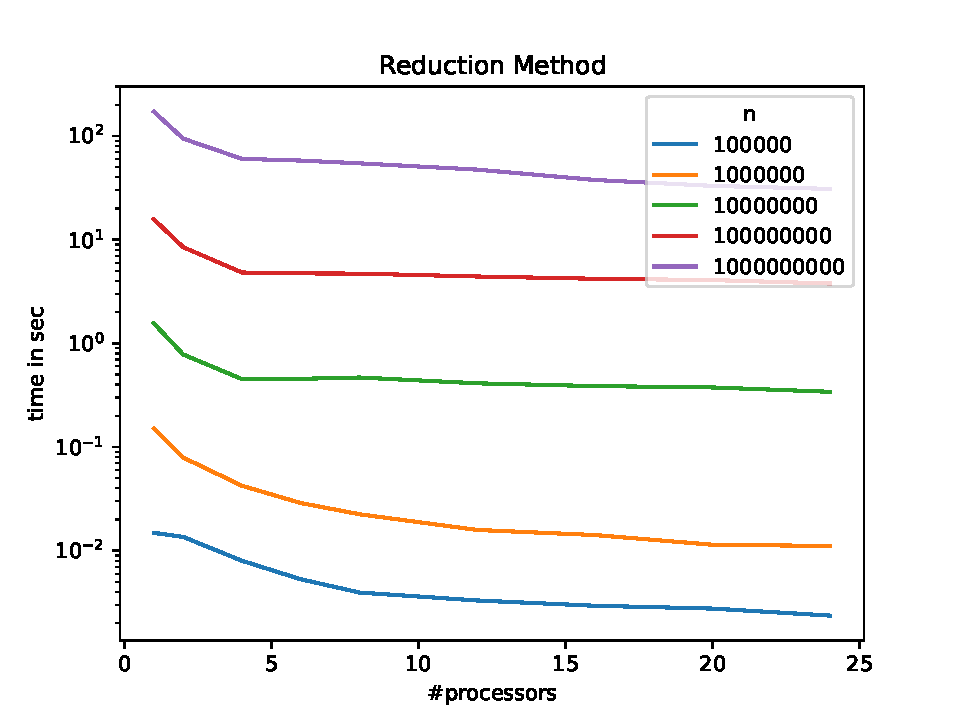
\includegraphics[width=0.3333\textwidth]{../results/perf_scaling_reduction.pdf}
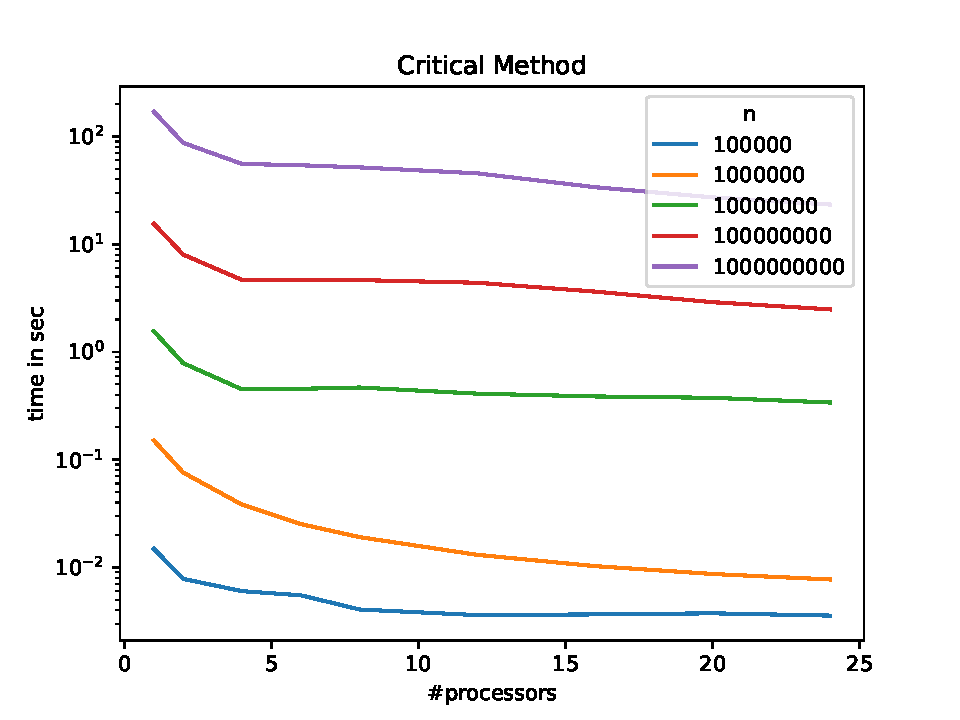
\includegraphics[width=0.3333\textwidth]{../results/perf_scaling_critical.pdf}
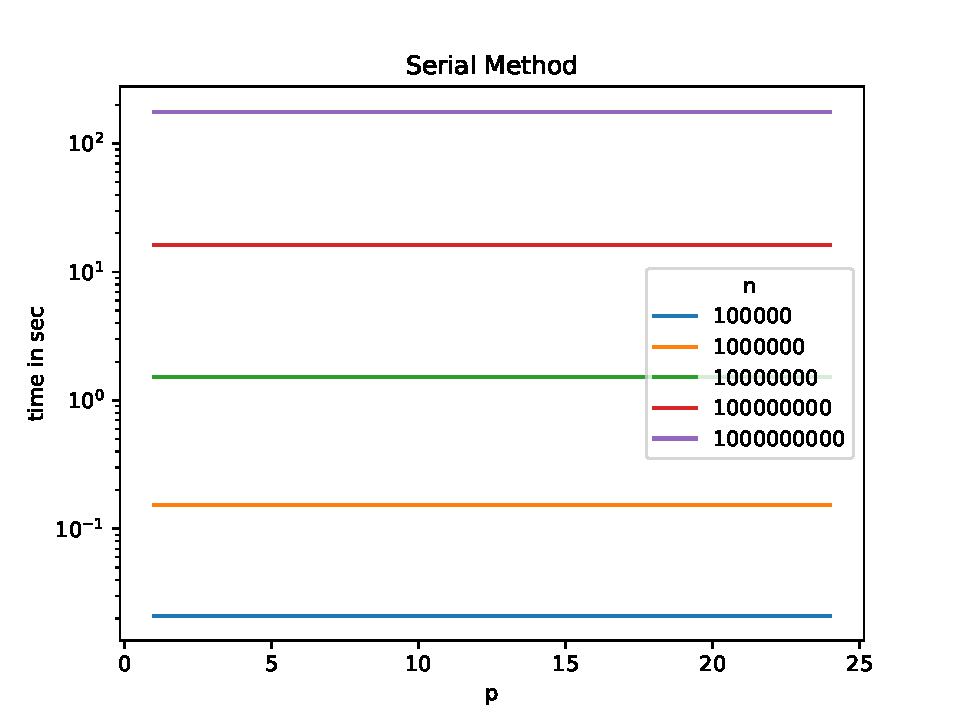
\includegraphics[width=0.3333\textwidth]{../results/perf_scaling_serial.pdf}

For the parallel plot we run the code for 1,2,4,6,8,12,16,20 and 24 threads. All three plots are the mean from 10 measurements.

% -------------------------------------------------------------------------- %
% -------------------------------------------------------------------------- %
% ---------------------- Exercise 2 -----------------------------------------%
% -------------------------------------------------------------------------- %
% -------------------------------------------------------------------------- %

\section{The Mandelbrot set using OpenMP [30 points]}

\subsection{Serial implementation}
The serial version of the code is implemented like the pseudocode on the projectdescription.

\subsection{Parallel implementation}
If we want to be sure about the values of \texttt{cx} and \texttt{cy} when parallelizing the loope we can not calculate theme the way they are in the serial version.
To avoid provlems we make \texttt{cx} and \texttt{cy} private variables and calculate them in the inner loop.
This lets us still use \texttt{cx} and \texttt{cy} for the calculations in the while loop.
Other variable which need to be private are \texttt{x},\texttt{y},\texttt{x2},\texttt{y2} as well as the new variable \texttt{n} which calculate the number of iterations for one complex number.
\texttt{n} is added to the public variable \texttt{nTotalIterationsCount} and to avoid race conditions we used \texttt{\#pragma omp atomic} for the calculation.

We only parallelized the outer loop with \texttt{\#omp pragma for} since we already have between 512 and 4096 iterations in this loop.
After trying different scheduels and blocksizes \texttt{schedule(dynamic)} and \texttt{schedule(static)} seem to run the best.
In this implementation we therefore us the dynamic schedule.

\subsection{Results}

As we can see in the plots our version does not scale at all. We were not able to figure out what the problem was and did not try it many times since the plots took multiple hours to run.

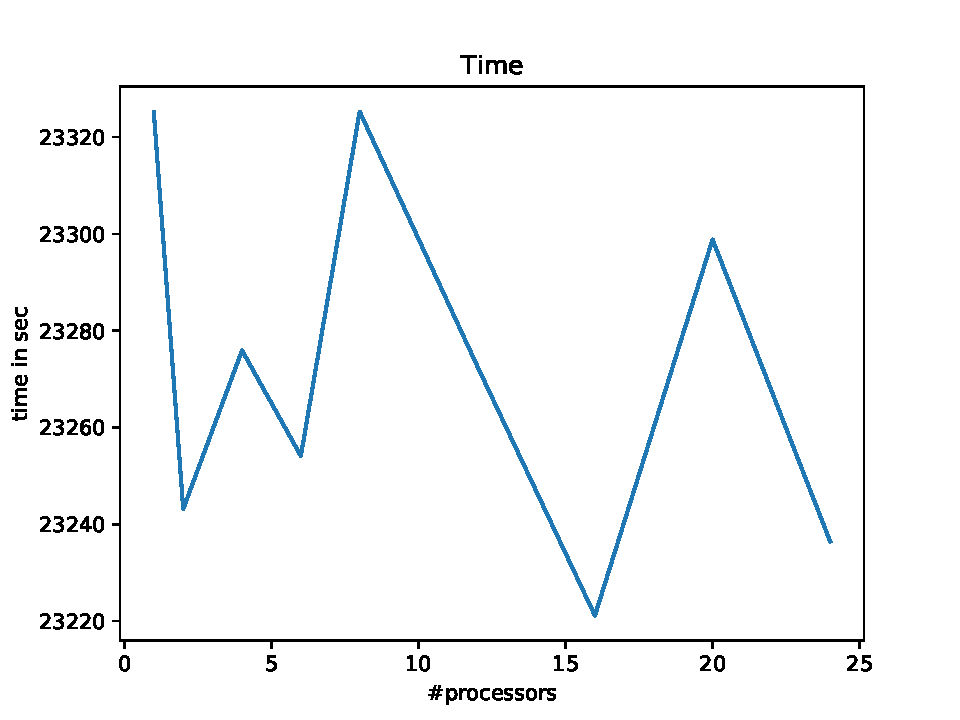
\includegraphics[width=0.33\textwidth]{../results/time.pdf}
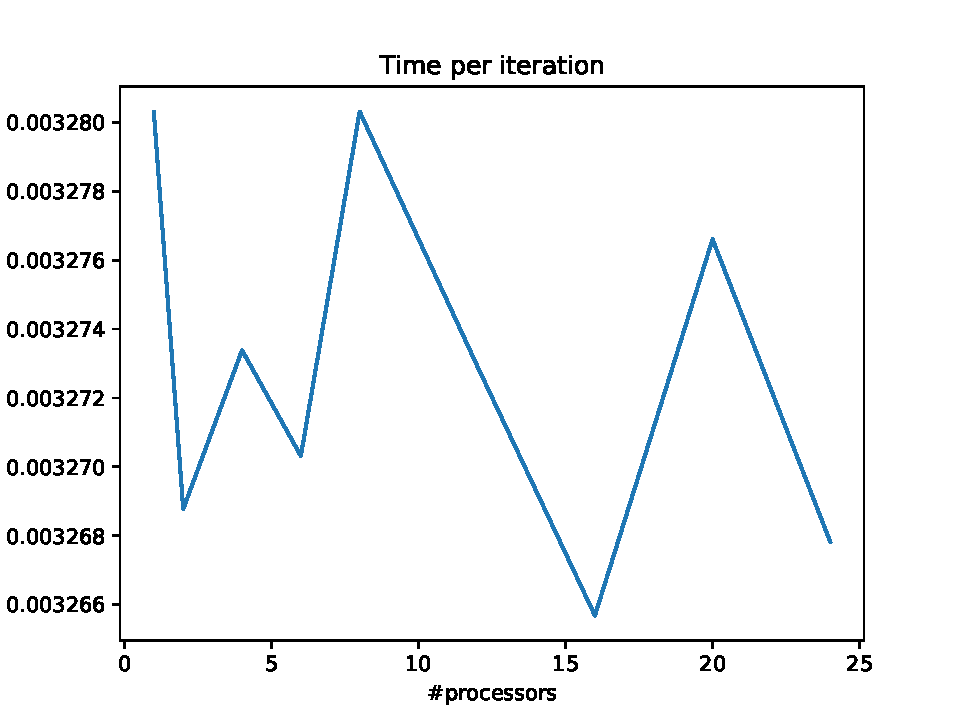
\includegraphics[width=0.33\textwidth]{../results/timeperiteration.pdf}
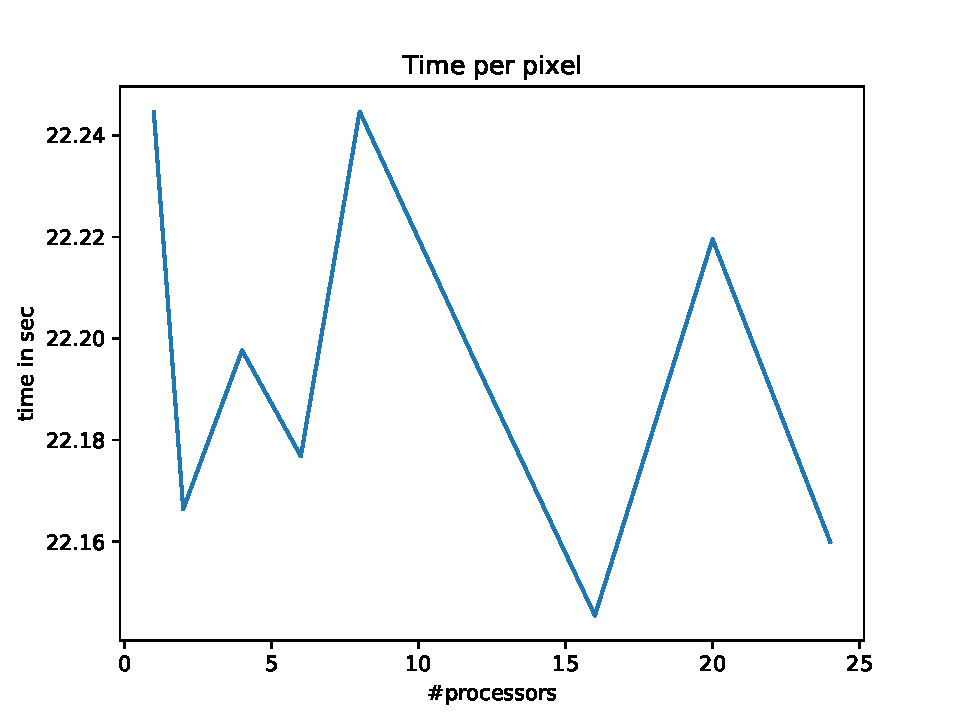
\includegraphics[width=0.33\textwidth]{../results/timeperpixel.pdf}


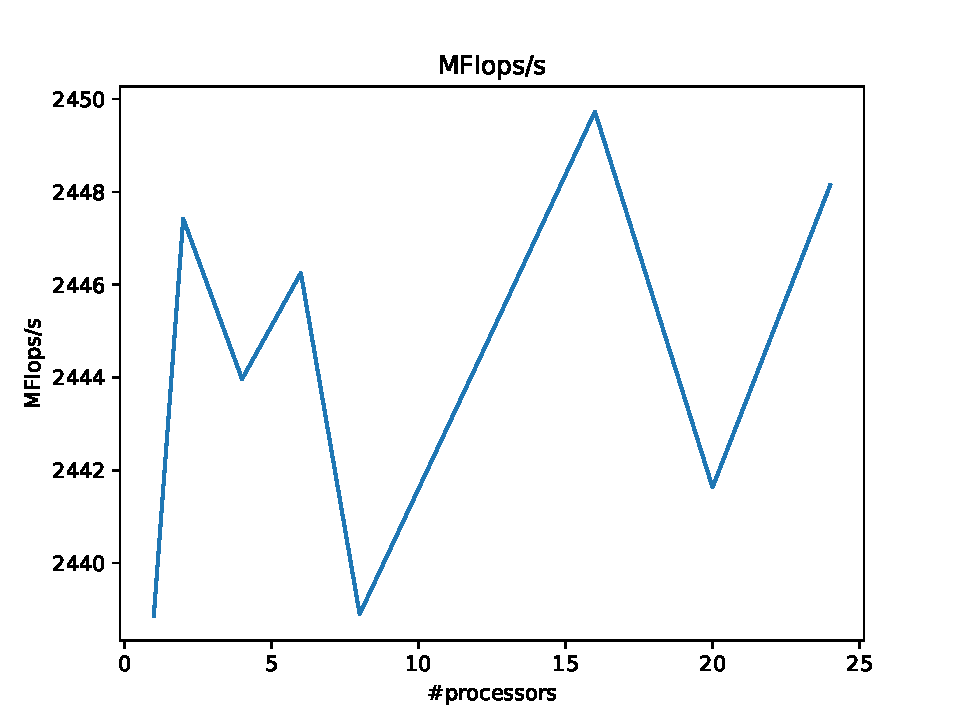
\includegraphics[width=0.33\textwidth]{../results/MFLops.pdf}
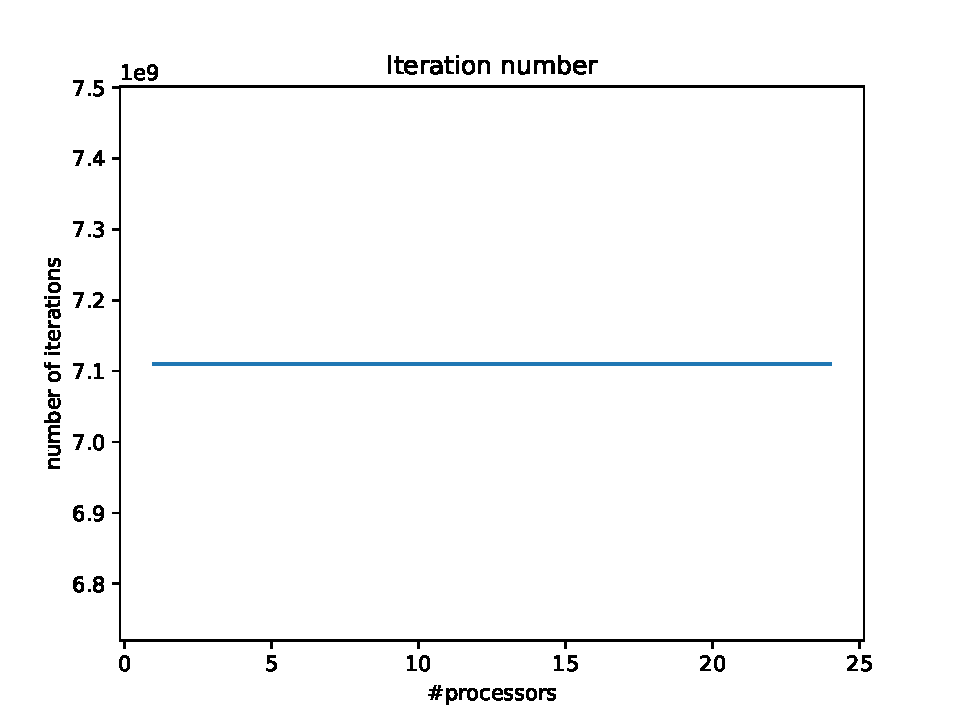
\includegraphics[width=0.33\textwidth]{../results/iterationnumber.pdf}
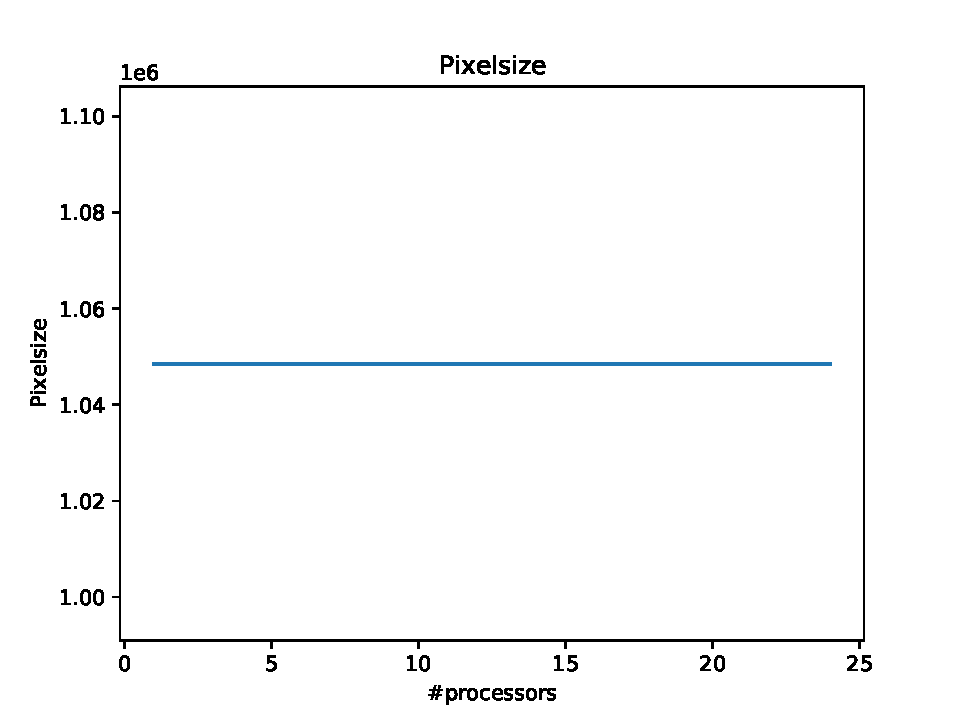
\includegraphics[width=0.33\textwidth]{../results/pixelsize.pdf}

For the parallel plot we run the code for 1,2,4,6,8,12,16,20 and 24 threads. The plots are the mean from 5 measurements.
We made plots for all the N values mentioned in the projectdescription but chose to present the ones from N = 1024 as a representative case. All the other plots look roughly the same.

% -------------------------------------------------------------------------- %
% -------------------------------------------------------------------------- %
% ---------------------- Exercise 3 -----------------------------------------%
% -------------------------------------------------------------------------- %
% -------------------------------------------------------------------------- %

\section{Bug hunt [15 points]}

\subsection{Bug 1}
\texttt{\#pragma omp parallel} and \texttt{\#pragma omp for} can only be combined, if the loop starts at the begin of the parallel region.
If there is any other code between the start of the parallel region and the for loop that needs to be parallelized
the \texttt{\#pragma omp for} needs to be in the parallel region directly before the for loop with no other code inbetween.
In this case we have \texttt{\#pragma omp parallel shared(a, b, c, chunk) private(i, tid)} as the initialization of the parallel region and 
\texttt{\#pragma omp for schedule(static, chunk)} right in front of the for loop.

\subsection{Bug 2}
The variable \texttt{tid} needs to be private since each thread needs to know its own id.
If it is public like in this case we dont know if we ever visit the if statement since at any time any thread can write his number to \texttt{tid}.
I also assumed, that we wanted to have the total for each thread and not the over all total. Therefore the variable \texttt{total} also needs to be private.
The solution would be to use \texttt{\#pragma omp parallel private(tid, total)}.
If we would want to know the total over all the thread the variable \texttt{total} would not be private.
Insted there would be a private variable \texttt{loc\_total} and we would calculate the local total over each thread.
At the end of the privat section we would add the \texttt{loc\_total} to \texttt{total} and make a critical section to avoit race contitions.

\subsection{Bug 3}
When using section in omp only one thread enters each section. In this program only threads entering a section call the print\_results function.
Since not all threads enter a section not all threads will call the print\_results function.
Because of this not all threads will reach the barrier in the print\_results function and the program stops.
This can be resolved by deleting the barrier in the print\_results function.
This is okey since it is the last part of each section and we have a barrier before we exit the sections nowait part.

\subsection{Bug 4}
The problem is, that the array a does not fit on the stack of each thread and we therefore get a segmentation fault.
Since a is private each thread needs enough memory to allocate a.
To avoid this we can give each thread more memory by calling "export OMP\_STACKSIZE="9M" " before executing the program.
For this size of a 9MB is enough since we have 1048*1048 doules and each double needs 8B of memory.
The stacksize we need to allocate therefore needs to be calculated new if the size of a changes.

\subsection{Bug 5}
In this code a deadlock occures because the thread in section 1 sets locka first and then wants to set lockb.
At the same time the thread in section 2 stes lockb and after initializing b tries to set locka.
This leads to a deadlock since both threads are waiting for the other thread to unset a lock.
To avoid this both threads need to set the first lock initialize their array and unset the lock.
Then both step set locka first and lockb secound add their array to the other array and then unlock both locks.
This prevents a deadlock because both threads unset their locks after initializing their array and then try to set the locks again in the same order.
For this example I assumed that the order in which the for loops get executed does not matter.

% -------------------------------------------------------------------------- %
% -------------------------------------------------------------------------- %
% ---------------------- Exercise 4 -----------------------------------------%
% -------------------------------------------------------------------------- %
% -------------------------------------------------------------------------- %


\section{Parallel histogram calculation using OpenMP [15 points]}

\subsection{Parallel implementation}
When looking at the for loop we need to parallelize we see, that each thread accesses a randomn location in the \texttt{dist} array.
Since having a critical region in each iteration of the for loop would make the code extremely slow we give each thread a local array \texttt{locdist}.
After the initialization of \texttt{locdist} we parallelize the for loop with \texttt{\#pragma omp for}.
Each thread adds the numbers up in to the local dist array. Before exiting the parallel region we add the numbers of the local dist arrays to the dist array.
To avoid race conditions we use the command \texttt{\#pragma omp atomic} when adding \texttt{locdist} to \texttt{dist}.

\subsection{Results}

As seen in the parallel runtime plot our solution scales well. The sequential code is even slower then the paralle version with 1 thread.
We are not sure why this is the case but we suspect that this is a measurement error.

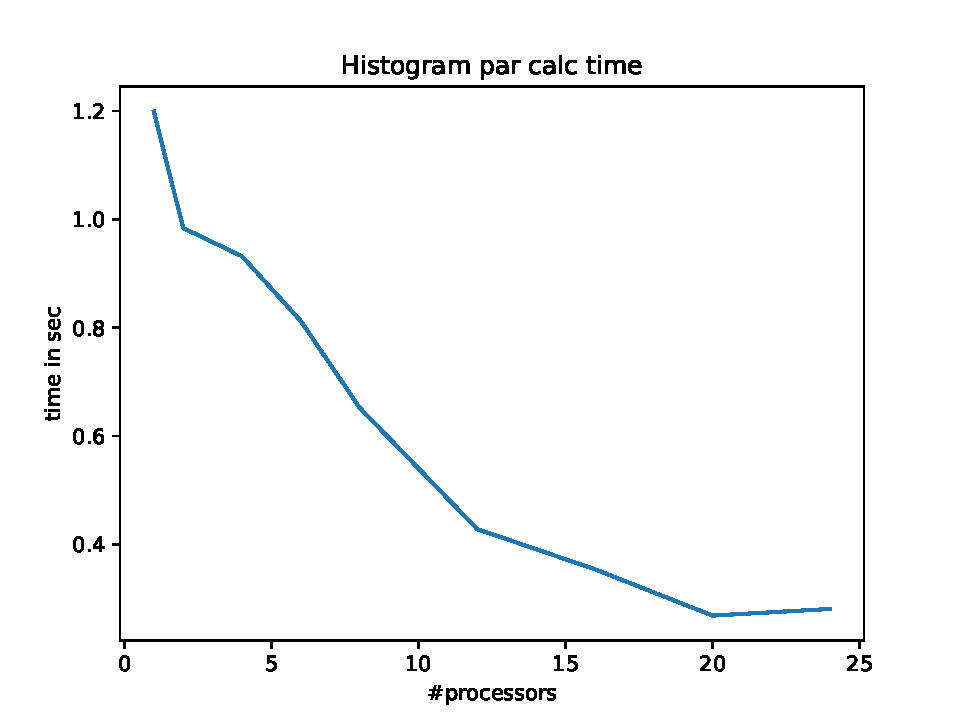
\includegraphics[width=0.5\textwidth]{../results/par_hist.pdf}
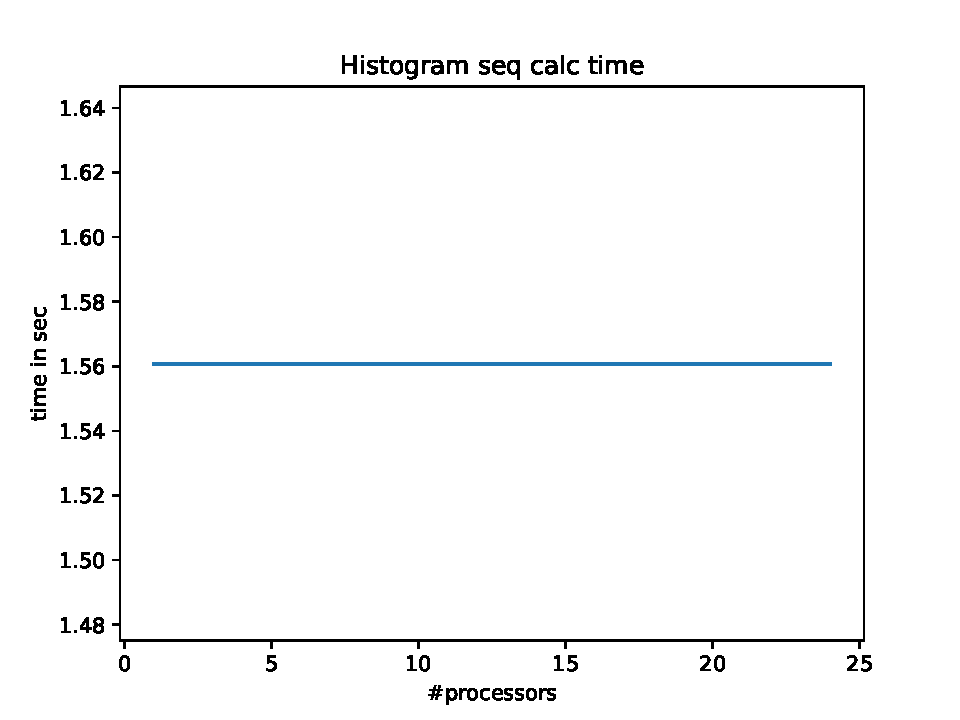
\includegraphics[width=0.5\textwidth]{../results/seq_hist.pdf}

For the parallel plot we run the code for 1,2,4,6,8,12,16,20 and 24 threads. The plots are the mean from 10 measurements.
The sequential plot is also the mean from 10 measurements.

% -------------------------------------------------------------------------- %
% -------------------------------------------------------------------------- %
% ---------------------- Exercise 5 -----------------------------------------%
% -------------------------------------------------------------------------- %
% -------------------------------------------------------------------------- %

\section{Parallel loop dependencies with OpenMP [15 points]}

\subsection{Parallel implementation}
The way we parallelize this for loop is by making a parallel region and giving each thread a block it has to calculate.
This ensures that each thread gets one connected block.
For the first element each thread calculates the start value with \texttt{pow(up,tid*N/nthreads) * Sn}.
Then the threads calculates the loop for its assigned block and saves the elements in the \texttt{opt} array.
For the parallelization of the loop we use reduction on the multiplication of \texttt{Sn}.

\subsection{Results}

As seen in the parallel runtime plot the solution scales very well. The parallel solution also only needs 5 seconds for one thread which is nearly as good as the serial solution.


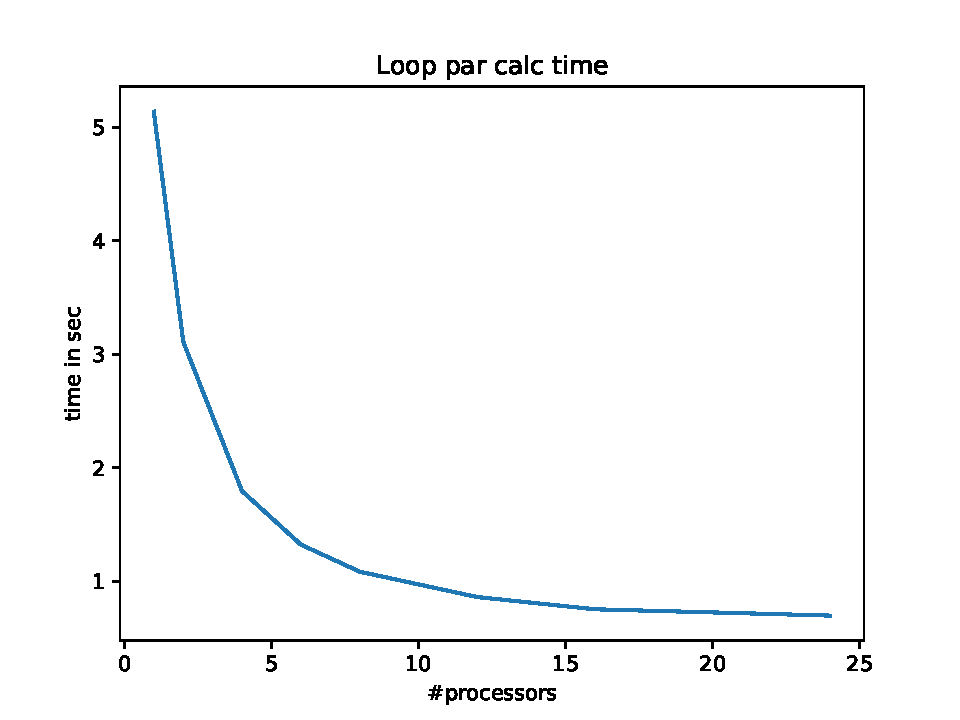
\includegraphics[width=0.5\textwidth]{../results/par_loop.pdf}
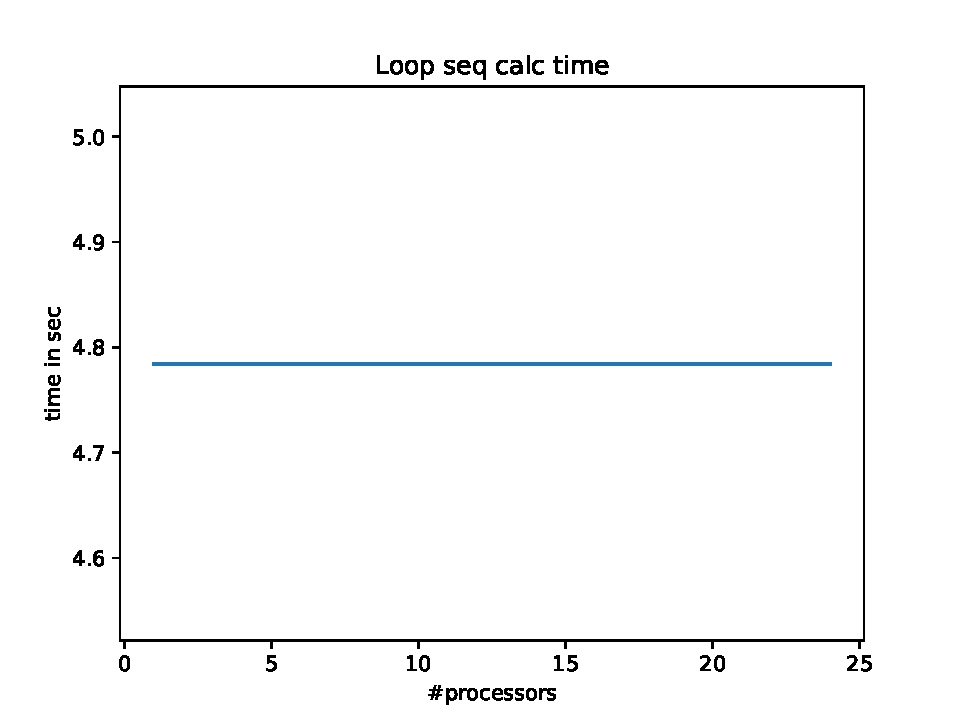
\includegraphics[width=0.5\textwidth]{../results/seq_loop.pdf}

For the parallel plot we run the code for 1,2,4,6,8,12,16,20 and 24 threads. The plots are the mean from 10 measurements.
The sequential plot is also the mean from 10 measurements.

\section{Task:  Quality of the Report   [15 Points]}


\section*{Additional notes and submission details}
Submit the source code files (together with your used \texttt{Makefile}) in
an archive file (tar, zip, etc.) and summarize your results and the
observations for all exercises by writing an extended Latex report.
Use the Latex template from the webpage and upload the Latex summary
as a PDF to \href{https://moodle-app2.let.ethz.ch/course/view.php?id=14316}{Moodle}.

\begin{itemize}
\item Your submission should be a gzipped tar archive, formatted like project\_number\_lastname\_firstname.zip or project\_number\_lastname\_firstname.tgz. 
      It should contain:
  \begin{itemize}
    \item all the source codes of your OpenMP solutions.
    \item your write-up with your name  project\_number\_lastname\_firstname.pdf, 
  \end{itemize}
   \item Submit your .tgz through Moodle.
  \end{itemize}



\end{document}
